% Requires \usepackage{tikz} and \usepackage{xcolor} in main.tex preamble

\chapter{The Book of the Practitioner}
\begin{center}
  \small\itshape The Constructive Text
\end{center}
\vspace{0.5em}
\begin{center}
  \itshape What you must be before what you must know.\\
  What you must do once you are both.
\end{center}
\vspace{1.5em}

\begin{center}
\small\itshape
This book is different from the rest of the gospel. The rest of the gospel names what is broken.\\
This book names what is whole. Read the rest first. Come here when you are ready to build.
\end{center}

% ============================================================
\section*{Part One: The Stack}
\addcontentsline{toc}{section}{Part One: The Stack}
\begin{center}
  \small\itshape Five layers. Each one earns the next. Most practitioners start at the bottom\\
  and assume the rest will follow. It does not follow.\\
  It has to be built, in order, from the inside out.
\end{center}
\vspace{2em}

% ============================================================
%  THE STACK DIAGRAM
%  Original triangle slope, shifted so the outer edge clips at the page.
%  Layer seams share y with the center-row gaps.
% ============================================================

% Requires \usepackage{tikz} and \usepackage{xcolor} in the preamble.
% Full-page-bleed Decision Stack: pyramids clip at the physical page edges.

\makeatletter
\definecolor{diag@gold}{RGB}{184,146,42}
\definecolor{diag@goldlt}{RGB}{212,168,67}
\definecolor{diag@dark}{RGB}{37,36,34}
\definecolor{diag@medium}{RGB}{64,61,57}
\definecolor{diag@light}{RGB}{204,197,185}
\definecolor{diag@cream}{RGB}{255,252,242}
\definecolor{diag@muted}{RGB}{90,80,64}
\makeatother

\vspace{0.5em}
\noindent
\makebox[\textwidth][l]{%
\hspace*{-\dimexpr\oddsidemargin+1in\relax}%
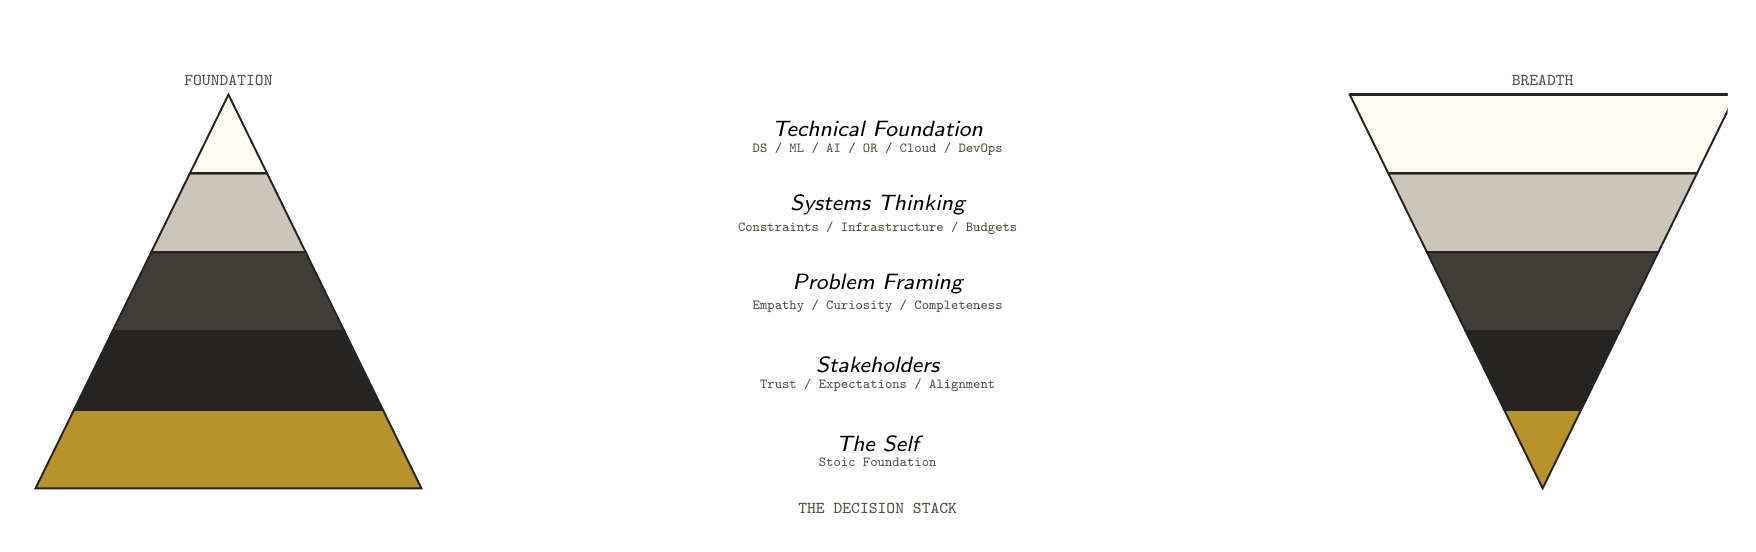
\begin{tikzpicture}[x=1cm, y=1cm, font=\sffamily]
  \pgfmathsetmacro{\W}{\paperwidth/1cm}
  \def\H{1.0}
  \pgfmathsetmacro{\Htot}{5*\H}
  % Foundation sits slightly closer to the labels than Breadth
  \pgfmathsetmacro{\hw}{2.45}
  \pgfmathsetmacro{\cxL}{2.55}
  \pgfmathsetmacro{\cxR}{\W-2.35}

  % Bounding box = clip window, so off-page vertices do not widen the picture
  \path[use as bounding box] (0,-0.45) rectangle (\W, 5.85);
  \clip (0,-0.45) rectangle (\W, 5.85);

  % ---- LEFT PYRAMID (upright; outer base bleeds off the left edge) ----
  \foreach \i/\lc in {1/diag@gold, 2/diag@dark, 3/diag@medium, 4/diag@light, 5/diag@cream} {
    \pgfmathsetmacro{\ybot}{(\i-1)*\H}
    \pgfmathsetmacro{\ytop}{\i*\H}
    \pgfmathsetmacro{\hwbot}{\hw*(1-\ybot/\Htot)}
    \pgfmathsetmacro{\hwtop}{\hw*(1-\ytop/\Htot)}
    \filldraw[fill=\lc, draw=diag@dark, line width=0.7pt, line join=miter]
      ({\cxL-\hwbot},\ybot) -- ({\cxL+\hwbot},\ybot) --
      ({\cxL+\hwtop},\ytop) -- ({\cxL-\hwtop},\ytop) -- cycle;
  }

  % ---- RIGHT PYRAMID (inverted; outer top bleeds off the right edge) ----
  \foreach \i/\lc in {1/diag@gold, 2/diag@dark, 3/diag@medium, 4/diag@light, 5/diag@cream} {
    \pgfmathsetmacro{\ybot}{(\i-1)*\H}
    \pgfmathsetmacro{\ytop}{\i*\H}
    \pgfmathsetmacro{\hwbot}{\hw*(\ybot/\Htot)}
    \pgfmathsetmacro{\hwtop}{\hw*(\ytop/\Htot)}
    \filldraw[fill=\lc, draw=diag@dark, line width=0.7pt, line join=miter]
      ({\cxR-\hwbot},\ybot) -- ({\cxR+\hwbot},\ybot) --
      ({\cxR+\hwtop},\ytop) -- ({\cxR-\hwtop},\ytop) -- cycle;
  }

  % Horizontal seams on top of each layer so cream/light read on white paper
  \foreach \i in {1,...,5} {
    \pgfmathsetmacro{\ytop}{\i*\H}
    \pgfmathsetmacro{\hwL}{\hw*(1-\ytop/\Htot)}
    \pgfmathsetmacro{\hwR}{\hw*(\ytop/\Htot)}
    \draw[diag@dark, line width=0.8pt]
      ({\cxL-\hwL},\ytop) -- ({\cxL+\hwL},\ytop);
    \draw[diag@dark, line width=0.8pt]
      ({\cxR-\hwR},\ytop) -- ({\cxR+\hwR},\ytop);
  }

  % Labels sit above each pyramid's center, which stays on the page
  \node[above, font=\fontsize{6}{7}\selectfont\ttfamily, text=diag@muted, inner sep=3pt]
    at (\cxL,\Htot) {FOUNDATION};
  \node[above, font=\fontsize{6}{7}\selectfont\ttfamily, text=diag@muted, inner sep=3pt]
    at (\cxR,\Htot) {BREADTH};

  % ---- CENTER TEXT COLUMN ----
  % Title sits just above the band midline, subtitle just below, so the pair
  % is tight and optically centered (a single \\ node sits too high).
  \foreach \ymid/\ttl/\sub in {
      4.43/{Technical Foundation}/{DS / ML / AI / OR / Cloud / DevOps},
      3.43/{Systems Thinking}/{Constraints / Infrastructure / Budgets},
      2.43/{Problem Framing}/{Empathy / Curiosity / Completeness},
      1.43/{Stakeholders}/{Trust / Expectations / Alignment},
      0.43/{The Self}/{Stoic Foundation}%
    } {
    \node[anchor=south, inner sep=1.2pt, outer sep=0pt, align=center]
      at ({\W/2}, \ymid)
      {\fontsize{8.5}{9}\selectfont\itshape \ttl};
    \node[anchor=north, inner sep=1.2pt, outer sep=0pt, align=center]
      at ({\W/2}, \ymid)
      {\fontsize{5.5}{6}\selectfont\ttfamily\color{diag@muted} \sub};
  }

  \node[anchor=north, font=\fontsize{6}{7}\selectfont\ttfamily, text=diag@muted,
        inner sep=2pt]
    at ({\W/2}, -0.12) {THE DECISION STACK};
\end{tikzpicture}%
}

\vspace{1.5em}

% ============================================================
%  PART ONE: STACK ENTRIES
% ============================================================

\entrylabel{The First Layer}
\subsection*{The Self}

\lettrine[lines=3, loversize=0.1, lraise=0.9]{E}{verything} in this book rests here.

Not technically. Not organizationally. Not in terms of credentials or years of experience or the particular flavor of advanced degree the industry currently rewards. Here. The Self. The layer nobody talks about at the conference. The layer that cannot be certified, cannot be put on a resume, cannot be demonstrated in a take-home assessment or a technical screen or a panel interview with three engineers and a product manager.

The layer that the work reveals anyway.

You are going to sit in rooms where the pressure to be wrong is enormous. Not wrong in the obvious way, not the way that gets corrected in a code review or a peer assessment. Wrong in the quiet way. The way where the senior person in the room has a preference and the preference is visible and the room is adjusting to it in real time and the adjustment feels like reading the room and the reading of the room feels like maturity and the maturity feels like professionalism and somewhere in all of that the honest answer got lost and nobody is going to name what happened because everyone is too comfortable with the result.

The practitioner without the first layer will adjust.

Not because they are dishonest. Because they have not done the work of knowing what they actually think, separate from what the room wants them to think. Because the two feel the same until you have practiced telling them apart. Because the practice is uncomfortable and the conference does not offer a session on it and the LinkedIn algorithm does not reward posts about it.

The Self is not a personality trait. It is not introversion or extroversion or confidence or any of the other things the industry uses as proxies for it. It is a practice. The specific practice of knowing your own biases before you encounter the problem, so that the problem can be seen clearly rather than through the particular distortion your history and your incentives and your desire to be liked and your fear of being wrong produce without your permission.

The Stoics called this the discipline of judgment. They meant: before you decide what the thing is, notice what you want the thing to be, and separate those two observations. The gap between them is where the honest work lives.

Marcus Aurelius practiced this in a notebook between battles. The congregation can practice it before the meeting. The specific practice is not complicated. It is simply the habit of asking, before the laptop opens, before the data pulls, before the recommendation is written: what do I want to be true here, and how is that different from what I can demonstrate to be true?

Most practitioners never ask.

Most practitioners produce answers their biases already knew, dressed in methodologies they learned afterward.

The first layer is the practice of being the kind of person who can be trusted to see the problem before constructing the solution. It is the hardest layer because it never finishes. There is no certificate. There is no milestone. There is only the meeting, and the frown, and the moment of choosing between the honest answer and the comfortable one, and whether the choice comes from somewhere solid or somewhere that shifts with the room.

\begin{center}\small\itshape
  Build this first. Build it always.\\
  The layers above depend on it and they know when it is not there.
\end{center}

% --------------------------------------------------------
\entrylabel{The Second Layer}
\subsection*{Stakeholders}

You cannot manage what you cannot see.

The second layer is the practice of seeing people clearly, which sounds obvious until you try to do it in a room where you need something from them, or where they have authority over your work, or where they have already decided what the answer should be and are waiting for you to confirm it.

The reason The Self comes first is not philosophical. It is practical. Your own need for approval is the primary obstacle to seeing stakeholders accurately. Your own fear of conflict is the primary reason you will hear what they want rather than what they need. Your own investment in a particular outcome is the primary reason you will manage them toward your answer rather than toward the truth.

The practitioner who has not done the first layer will walk into the stakeholder conversation already compromised. They will hear the preferences and call them requirements. They will sense the resistance and route around it rather than surfacing it. They will present the work to the person they wish the stakeholder was rather than the person the stakeholder is, which means the work will land wrong and they will call it a communication problem.

It is not a communication problem. It is a seeing problem.

The stakeholder layer is not about being liked. The congregation should write this somewhere visible. The goal is not a warm relationship. The goal is an accurate model of what the stakeholder actually needs, what they will actually do with the output, what constraints they are operating under that they have not named, what fears they have about the work that they have expressed as objections, and what they need to believe in order to act on the recommendation when it arrives.

All of that is invisible if you walk in wanting to be approved of.

The practitioner with the second layer asks different questions. Not \textit{what do you want the answer to be}, but \textit{what decision are you trying to make and what would change for you if you made it differently.} Not \textit{how can I make this easier to accept}, but \textit{what would make this impossible to ignore.} Not \textit{what do you already believe}, but \textit{what would you need to see to believe something different.}

\begin{center}\small\itshape
  The second layer is built on the first.\\
  It cannot be built without it.
\end{center}

% --------------------------------------------------------
\entrylabel{The Third Layer}
\subsection*{Problem Framing}

The layer where most projects are decided before anyone knows it.

By the time you reach this layer, the work the first two layers did is either present or it is not, and the framing will show which. The practitioner with a solid foundation will frame the problem as it actually is. The practitioner without one will frame the problem as it is convenient to frame, or as the stakeholder wants it framed, or as the previous project framed it because the previous project is the only template available and starting from scratch is uncomfortable.

Problem framing is not a technique. The congregation has been told it is a technique. The congregation has been given templates and canvases and workshops designed to produce a frame at the end of a structured process. These tools are not wrong. They are just insufficient when the person using them has not done the first two layers, because a template cannot compensate for a practitioner who does not know their own biases and cannot see their stakeholders clearly.

The honest frame has four elements. Not as a template. As a discipline.

The decision. The specific, attributable, consequential choice that a real person will make differently because this work was done. If you cannot name it in one sentence, the frame is not finished.

The measure. What does better look like, specifically. Not a metric that will make leadership comfortable. The actual thing that changes in the world when the decision is made correctly.

The uncertainty. What do we not know, and how much does not knowing it cost. This is the element most likely to be removed before the deck is presented. It should be the element most carefully preserved. The uncertainty is not a failure of the analysis. The uncertainty is part of the answer.

The tradeoffs. What does this decision cost, and who bears the cost, and have those people been consulted. The frame that has no tradeoffs is the frame that has not been finished.

\begin{center}\small\itshape
  The third layer is where the Six Steps begin.\\
  Everything below it was preparation. This is the work.
\end{center}

% --------------------------------------------------------
\entrylabel{The Fourth Layer}
\subsection*{Systems Thinking}

The layer where the solution meets the world it has to live in.

By now the decision is named. The stakeholders are understood. The frame is honest. And the practitioner turns to face the actual environment where the work will be deployed, which is never the clean environment the frame implied and is always messier, more constrained, more politically complicated, more technically fragile, and more resistant to change than any model of it will capture.

Systems thinking is not a soft skill. The congregation should push back on anyone who calls it that. Systems thinking is the disciplined practice of understanding how the parts of a complex environment interact, where the leverage points are, where the constraints bind, what happens downstream when you push something upstream, and why the obvious intervention almost always produces unintended consequences that the obvious intervention was not designed to handle.

The fourth layer is where constraints become inputs rather than obstacles. Budget is not a reason to abandon the work. Budget is a dimension of the problem. Timeline is not a limitation on quality. Timeline is a constraint that reshapes what quality looks like in this specific context. Organizational resistance is not a failure of communication. Organizational resistance is data about the system that the solution has to survive inside.

The practitioner with the fourth layer does not build in the abstract. They build for the specific, complicated, politically real environment the solution will be deployed into, and they factor that environment into every design decision from the beginning rather than discovering it at the end when it is too late to do anything except apologize for the mismatch.

\begin{center}\small\itshape
  Every model of a system is a simplification.\\
  The question is not whether the simplification is perfect. It never is.\\
  The question is whether it preserves the features that matter for the decision at hand.
\end{center}

% --------------------------------------------------------
\entrylabel{The Fifth Layer}
\subsection*{Technical Foundation}

The layer the industry mistakes for the whole stack.

Technical foundation is real and necessary and enormously complex. Data science, machine learning, artificial intelligence, operations research, cloud infrastructure, software engineering. Each domain is vast. Each has subcategories that are themselves vast. The interactions between them are genuinely complicated in ways that take years to understand and years more to apply well.

And it is the least important layer on this list.

Not because it is easy. It is not easy. Not because it does not matter. It matters enormously. Because it is the most learnable layer, and because learning it in the absence of the layers above it produces exactly the problem the rest of this gospel has been diagnosing: technically correct work that answers the wrong question, at scale, with confidence, deployed into an organization that does not understand it and cannot use it correctly.

The tragedy of the current era is not that practitioners lack technical skills. The practitioners are technically skilled. The tragedy is that the industry selects for, trains for, recruits for, promotes for, and celebrates technical skill while treating the four layers above it as soft, optional, unteachable, or already handled.

They are not already handled.

They are never handled by default. They are built, deliberately, by practitioners who understood that the technical layer is the floor and not the ceiling, and who did the harder work of building everything above it.

The practitioner who has built all five layers arrives at a technical problem differently than the practitioner who has only built one. They arrive knowing what the work is for. Knowing who it serves. Knowing how the solution will live in the world. Knowing what they want to be true and what the evidence actually says. The technical foundation, in those hands, produces something the foundation alone never could.

\begin{center}\small\itshape
  Build the foundation. It is necessary.\\
  Do not stop there.
\end{center}

% ============================================================
\section*{Part Two: The Six Steps}
\addcontentsline{toc}{section}{Part Two: The Six Steps}
\begin{center}
  \small\itshape The cycle the prepared practitioner runs. Not a checklist. A discipline.\\
  The steps exist to be returned to, not completed.
\end{center}
\vspace{1.5em}

% --------------------------------------------------------
\entrylabel{Step One}
\subsection*{The Metaproblem}

Before the problem, there is a harder problem.

The metaproblem is the question of whether this is the right thing to be working on. Not whether the project is well-defined. Not whether the team has the capability. Whether this, among everything the organization could be doing, among everything this practitioner could be working on, is the problem that most deserves the work.

Most practitioners never ask this question. It is not asked at the kickoff. It is not on the project charter template. It is not what the stakeholder wants to spend the first meeting on. The stakeholder wants to spend the first meeting on timeline and scope and deliverables and team composition, because those things feel like progress and the metaproblem feels like delay.

The metaproblem is not delay. The metaproblem is the only question that makes the rest of the work honest.

The practitioner who skips it will build the right solution to the wrong problem, beautifully, on time, under budget, and will stand at the ribbon cutting watching the bridge connect nothing to nothing and will not understand why.

The metaproblem requires the full stack. It requires self-knowledge because the practitioner's own interests and biases shape which problems look important. It requires stakeholder understanding because the problem as presented is never the problem as it actually exists. It requires framing discipline because a poorly framed metaproblem produces a well-executed project aimed at the wrong target. It requires systems thinking because the right problem to work on is always the one whose solution propagates most usefully through the system.

\begin{center}\small\itshape
  Ask it. Even when the room is impatient. Even when the timeline is already set.\\
  Even when the project has a name and a budget and a sponsor and a Slack channel.\\
  Especially then.
\end{center}

% --------------------------------------------------------
\entrylabel{Step Two}
\subsection*{Frame the Problem}

The step most likely to be skipped.

The skip has been named elsewhere in this gospel. It lives here. This is its home. The specific moment when the room has the data open and the stakeholders are assembled and the timeline is visible and the pressure to produce is at its highest and the frame has not been agreed on and someone opens the laptop and the frame drifts away unspoken and the project begins.

The frame is the decision. The measures. The uncertainty. The tradeoffs. All four, written down, agreed upon, connected to a specific person who will act on the output, before a single query is written.

The frame is not a document. Documents can be produced without doing the framing. Forms can be filled out while skipping the substance. The frame is an agreement, between the practitioner and the decision maker, about what the work is for and what success looks like and what happens when the work is done.

That agreement requires two things the template cannot provide. A decision maker who is present, engaged, and willing to be specific about what they actually need. And a practitioner who is prepared, by everything in Part One of this book, to hear the honest answer without filtering it through what they want to hear.

\begin{center}\small\itshape
  Frame anyway. With whatever you have.\\
  Imperfect framing is better than no framing.\\
  A frame that gets revised is better than a frame that was never built.
\end{center}

% --------------------------------------------------------
\entrylabel{Step Three}
\subsection*{Solutioning}

Design constrained by feasibility.

Not design constrained by what is technically interesting. Not design constrained by what was done on the last project. Not design constrained by the tools that are already licensed or the methods that are already familiar or the solution that the practitioner knew they were going to build before the frame was finished.

Design constrained by feasibility. By what will actually work in the actual environment for the actual decision maker with the actual data and the actual timeline and the actual organizational will to change.

This is the step where technical foundation earns its seat at the table. The practitioner who has built all five layers arrives here with a clear frame, an accurate picture of the stakeholder, an honest understanding of their own biases, and a working model of the system the solution has to survive in. Technical depth in those hands is not decoration. It is the toolkit applied to a well-defined problem.

The congregation should note what changes at this step when the stack is incomplete. The practitioner without self-knowledge will design toward the solution they prefer rather than the solution the problem requires. The practitioner without stakeholder understanding will design for the wrong user. The practitioner without framing discipline will design something technically correct that addresses the adjacent problem. The practitioner without systems thinking will design something that works in isolation and fails in context.

\begin{center}\small\itshape
  The elegance of the design is not the measure.\\
  The measure is whether the design serves the frame.\\
  If it requires the frame to change, go back to Step Two. That is not failure.\\
  That is solutioning working correctly.
\end{center}

% --------------------------------------------------------
\entrylabel{Step Four}
\subsection*{Data}

Source it or re-solution.

The step the industry starts at is the fourth step. This is worth stating plainly one more time, not because the congregation does not know it but because the congregation works in organizations that do not know it and the repetition is useful armor for the rooms the congregation has to survive.

Data is not the beginning. Data is the fourth step. It arrives after the decision has been named, after the frame has been built, after the solution has been designed. It arrives knowing what it is for, which is the condition under which data is actually useful rather than merely present.

The data audit has two outcomes and only two. Either the data needed to support the solution exists and is accessible and is sufficiently clean, in which case the project proceeds. Or it does not, in which case the project does not proceed in the direction it was heading and the practitioner returns to Step Three to design a solution that works with the data that actually exists.

This is not a setback. This is the discipline working correctly. A solution designed around available data is not a compromise. It is an honest solution. A solution designed around ideal data that does not exist is a fantasy dressed in methodology.

\begin{center}\small\itshape
  Treat absence as a constraint. Re-solution around it.\\
  The frame survives. The solution changes. The work continues.
\end{center}

% --------------------------------------------------------
\entrylabel{Step Five}
\subsection*{Build}

From proof of concept to pilot to minimum viable product to production.

Each stage is a question, not a milestone. The proof of concept asks: does this approach work at all? The pilot asks: does it work in the real environment with real users and real data and real constraints? The MVP asks: does it work well enough to be acted on? Production asks: is it working, and is the thing it is working on still the right thing?

The build step is where adoptable beats optimal. The congregation has heard this before. It bears repeating here because the build step is where the temptation to optimize for correctness rather than adoption is strongest. The model is in front of the practitioner. The model is good. The model is better than the version that will actually get used. The temptation is to keep building the better version rather than shipping the good enough one.

Ship the good enough one.

The better version that sits on a laptop serves no decision. The good enough version that gets used, that practitioners trust, that decision makers act on, that produces outcomes that can be measured and improved, is the whole point. The better version is a private satisfaction. The used version is the discipline.

\begin{center}\small\itshape
  Build for the person who will use it. Not the person you wish would use it.\\
  Not the organization you wish this was. The actual person, with the actual constraints,\\
  in the actual system.\\
  That constraint is not a limitation on the work. It is the most important specification the work has.
\end{center}

% --------------------------------------------------------
\entrylabel{Step Six}
\subsection*{Return}

All the way back to Step One.

Not as failure. Not as retreat. As the discipline completing its cycle and beginning again with everything the previous cycle taught.

The return is the step that separates the practitioner from the project manager. The project manager delivers and moves on. The practitioner delivers and asks whether the delivery served the decision, whether the decision is still the right decision, whether the system around the decision has changed enough that the whole frame needs to be revisited.

The return is also the step the Fourth Horseman depends on never happening. The orphaned decision system is the system whose practitioners never returned to Step One. They built it, shipped it, declared it complete, and moved to the next project, and the system ran and ran and ran until the decision it was built to support had changed and nobody had noticed because nobody's job was to notice.

Make it someone's job to notice.

The return is not scheduled on the project timeline. The return does not appear in the statement of work. The return is the practitioner's own commitment to the work, sustained past the delivery, past the celebration, past the moment when everyone has moved on to something new and the system is running quietly in production serving a decision that may or may not still be the right decision to serve.

Return.

Ask the question.

\textit{Does this still make sense?}

The answer is sometimes yes and the work continues. The answer is sometimes no and the cycle begins again. The answer is never obvious without asking, which is why so few practitioners ask, which is why so many systems run past their usefulness quietly costing the organization something it cannot see.

\begin{center}\small\itshape
  Return is not the last step.\\
  Return is how the discipline stays alive.
\end{center}

% ============================================================
%  CLOSING
% ============================================================

\vspace{2em}
\sermonrule

\subsection*{The Closing of the Book of the Practitioner}

\lettrine[lines=3, loversize=0.1, lraise=0.9]{T}{he} stack and the cycle are one thing.

They look like two things because they are described in sequence, the stack first and then the steps, but the sequence is pedagogical, not operational. In practice they are simultaneous. The step you are on reveals which layer of the stack is under stress. The layer of the stack that is weak shapes which step will fail.

The practitioner who has the Self but not the systems thinking will frame brilliantly and solution naively. The practitioner who has the technical foundation but not the stakeholder layer will build precisely and deliver uselessly. The practitioner who has all five layers but will not return to Step One has built something that will become a monument when it should have remained a tool.

The discipline is not a destination. The congregation should have understood this from Genesis. The discipline is a practice, which means it is the thing you do every day in every room with every problem, and the doing of it is the whole of it, and the day you stop doing it is the day the work starts serving your preferences rather than the decision.

\begin{closingverse}
  The stack is what you must be.\\
  The steps are what you must do.\\
  Neither is sufficient alone.\\[0.8em]
  \upshape Together they are the whole practice.
\end{closingverse}
